\documentclass[aspectratio=169,xcolor={dvipsnames,table}]{beamer}
\usepackage[no-math,deluxe,haranoaji]{luatexja-preset}
\renewcommand{\kanjifamilydefault}{\gtdefault}
\renewcommand{\emph}[1]{{\upshape\bfseries #1}}
\usetheme{metropolis}
\metroset{block=fill}
\setbeamertemplate{navigation symbols}{}
\setbeamertemplate{blocks}[rounded][shadow=false]
\usecolortheme[rgb={0.7,0.2,0.2}]{structure}
%%%%%%%%%%%%%%%%%%%%%%%%%%
%% Change alert block colors
%%% 1- Block title (background and text)
\setbeamercolor{block title alerted}{fg=mDarkTeal, bg=mLightBrown!45!yellow!45}
\setbeamercolor{block title example}{fg=magenta!10!black, bg=mLightGreen!70}
%%% 2- Block body (background)
\setbeamercolor{block body alerted}{bg=mLightBrown!25}
\setbeamercolor{block body example}{bg=mLightGreen!15}
%%%%%%%%%%%%%%%%%%%%%%%%%%%
\usepackage[absolute,overlay]{textpos}
\usepackage[grid=true,gridcolor=Maroon,subgridcolor=gray,gridunit=pt,texcoord]{eso-pic} %場所決めのためのgrid表示
%%%%%%%%%%%%%%%%%%%%%%%%%%%
%% さまざまなアイコン
%%%%%%%%%%%%%%%%%%%%%%%%%%%
%\usepackage{fontawesome}
\usepackage{fontawesome5}
\usepackage{figchild}
\usepackage{twemojis}
\usepackage{utfsym}
\usepackage{bclogo}
\usepackage{marvosym}
\usepackage{fontmfizz}
\usepackage{pifont}
\usepackage{phaistos}
\usepackage{worldflags}
\usepackage{jigsaw}
\usepackage{tikzlings}
\usepackage{tikzducks}
\usepackage{scsnowman}
\usepackage{epsdice}
\usepackage{halloweenmath}
\usepackage{svrsymbols}
\usepackage{countriesofeurope}
\usepackage{tipa}
%%%%%%%%%%%%%%%%%%%%%%%%%%%
\usepackage{tikz}
\usetikzlibrary{calc,patterns,decorations.pathmorphing,backgrounds}
\usepackage{tcolorbox}
\usepackage{tikzpeople}
\usepackage{circledsteps}
\usepackage{xcolor}
\usepackage{amsmath}
\usepackage{booktabs}
\usepackage{chronology}
\usepackage{signchart}
%%%%%%%%%%%%%%%%%%%%%%%%%%%
%% 場合分け
%%%%%%%%%%%%%%%%%%%%%%%%%%%
\usepackage{cases}
%%%%%%%%%%%%%%%%%%%%%%%%%%
\usepackage{pdfpages}
%%%%%%%%%%%%%%%%%%%%%%%%%%%
%% 音声リンク表示
\newcommand{\myaudio}[1]{\href{#1}{\faVolumeUp}}
%%%%%%%%%%%%%%%%%%%%%%%%%%
%% \myAnch{<名前>}{<色>}{<テキスト>}
%% 指定のテキストを指定の色の四角枠で囲み, 指定の名前をもつTikZの
%% ノードとして出力する. 図には remember picture 属性を付けている
%% ので外部から参照可能である.
\newcommand*{\myAnch}[3]{%
  \tikz[remember picture,baseline=(#1.base)]
    \node[draw,rectangle,line width=1pt,#2] (#1) {\normalcolor #3};
}
%%%%%%%%%%%%%%%%%%%%%%%%%%
%% \myEmph コマンドの定義
%%%%%%%%%%%%%%%%%%%%%%%%%%
%\newcommand{\myEmph}[3]{%
%    \textbf<#1>{\color<#1>{#2}{#3}}%
%}
\usepackage{xparse} % xparseパッケージの読み込み
\NewDocumentCommand{\myEmph}{O{} m m}{%
    \def\argOne{#1}%
    \ifx\argOne\empty
        \textbf{\color{#2}{#3}}% オプション引数が省略された場合
    \else
        \textbf<#1>{\color<#1>{#2}{#3}}% オプション引数が指定された場合
    \fi
}
%%%%%%%%%%%%%%%%%%%%%%%%%%%
%%%%%%%%%%%%%%%%%%%%%%%%%%%
%% 文末の上昇イントネーション記号 \myRisingPitch
%% 通常のイントネーション \myDownwardPitch
%% https://note.com/dan_oyama/n/n8be58e8797b2
%%%%%%%%%%%%%%%%%%%%%%%%%%%
\newcommand{\myRisingPitch}{
\begin{tikzpicture}[scale=0.3,baseline=0.3]
\draw[->,>=stealth] (0,0) to[bend right=45] (1,1);
\end{tikzpicture}
}
\newcommand{\myDownwardPitch}{
\begin{tikzpicture}[scale=0.3,baseline=0.3]
\draw[->,>=stealth] (0,1) to[bend left=45] (1,0);
\end{tikzpicture}
}
%%%%%%%%%%%%%%%%%%%%%%%%%%%%
%\AtBeginSection[%
%]{%
%  \begin{frame}[plain]\frametitle{授業の流れ}
%     \tableofcontents[currentsection]
%   \end{frame}%
%}

\usepackage{pxrubrica}
\usetikzlibrary{tikzmark}
%%%%%%%%%%%%%%%%%%%%%%%%%%%
\title{English is fun.}
\subtitle{I know that she is kind.}
\author{}
\institute[]{}
\date[]

%%%%%%%%%%%%%%%%%%%%%%%%%%%%
%% TEXT
%%%%%%%%%%%%%%%%%%%%%%%%%%%%
\begin{document}

\begin{frame}[plain]
  \titlepage
\end{frame}

\section*{授業の流れ}
\begin{frame}[plain]
  \frametitle{授業の流れ}
  \tableofcontents
\end{frame}

%%%%%%%%%%%%%%%%%%%%%%%%%%%%%%%%%%%%%%%%%%%%%
\section{that \textipa{/D@t/}}
\subsection{接続詞that}
%%%%%%%%%%%%%%%%%%%%%%%%%%%%%%%%%%%%%%%%%%%%%
\begin{frame}[plain,t]{S $+$ V \fbox{that s $+$ v}}
\large
\begin{enumerate}
 \item I know George.\hfill{\scriptsize Georgeは目的語(O)}
 \item I know the fact.\hfill{\scriptsize fact \textipa{/f\'\ae kt/} 事実}
 \item I know \fbox{\textbf{that} she is kind}.\hfill{}{\small \textbf{S} $+$ \textbf{V}\,\,\,\fbox{\textbf{that} \textbf{s} $+$ \textbf{v}}\,\,($=$ O)}
\end{enumerate}

\vspace{30pt}

\begin{block}{Topics for Today}\small
\begin{itemize}\setbeamertemplate{items}[square]\small
 \item   \Circled[fill color = white]{\,\,\textbf{that}  {\bfseries s $+$ v}\,\,}\,\,は「〜ということ」という意味
 \item   \Circled[fill color = white]{\,\,\textbf{that} {\bfseries s $+$ v}\,\,}\,\,は全体で「名詞」の役割
 \item  {\bfseries S$_1$ $+$ V$_1$}\,\,\,\,\Circled[fill color=white]{\,\,\tikzmark{oyoyo}\textbf{that}\,\,{\bfseries s$_2$ $+$ v$_2$}\,\,}
\\
\mbox{}\hfill{\scriptsize \tikzmark{piyo}この\textbf{that}は\kenten{接続詞}です}
\end{itemize}
     \end{block}

\vspace{-10pt}

\hfill{\tiny 0132}\,{\scriptsize \myaudio{./audio/054_that_clause_01.mp3}}


\begin{tikzpicture}[remember picture,overlay]
 \visible{\draw[<-] ([xshift=8pt,yshift=-4pt] pic cs:oyoyo) |- ([xshift=-2pt, yshift=2pt] pic cs:piyo);}
\end{tikzpicture}
\end{frame}
%%%%%%%%%%%%%%%%%%%%%%%%
\section{直後にthat S $+$ Vを従える動詞}
%%%%%%%%%%%%%%%%%%%%%%%%%%%%
\begin{frame}[plain,label=ichiran]{直後に\fbox{that S $+$ V}を従える動詞}
 \bfseries\large
\hfill{}S $+$ $\left\{
\begin{tabular}{l}
 know\\
 believe\\
 hope\\
 think\\
 say
\end{tabular}
\right\}$
\,\,\,\fbox{that\,\,\,\,S $+$ V}\hfill\hfill\mbox{}

\normalsize
\begin{textblock*}{0.4\linewidth}(320pt,100pt)
\visible<1->{\begin{tikzpicture}
\chicken[
scale=1.4141,
%speech={\tiny  be動詞},
signpost=\scalebox{.5}{
\parbox{3cm}{\color{black}
\centering know, think, believeなど\\認識・思考を表す動詞が多い!}},
signcolour= brown!70!gray,
signback=white!80!brown
]
\end{tikzpicture}}
\end{textblock*}
\end{frame}
%%%%%%%%%%%%%%%%%%%%%%%%%%%%
\begin{frame}[plain,t]{直後に\fbox{that S $+$ V}を従える動詞}
 \centering
\vspace*{20pt}
\begin{tblr}{
  colspec={llll},
  row{1} = {font=\bfseries},
  hline{1,Z}={0.08em},
  hline{2}={0.05em},
  row{even}={bg=Yellow!50},
%  row{7-8}={bg=NavyBlue!30},
%  row{9}={bg=Maroon!20},
  cells={cmd=\onslide<\arabic{rownum}->}
}
     原形  & 過去形   & 過去分詞&  例文    \\
know  & knew & known& We \textbf{know that} the Earth is round.   \\
believe & believed   & believed & She \textbf{believes that} he will succeed.    \\
hope  & hoped  & hoped& We \textbf{hope that} she will win the game.    \\
think        & thought   & thought&  I \textbf{think that} she will come.     \\
say    & said   & said&  She \textbf{said that} he was kind.
\end{tblr}

\hfill{\tiny 0229}\,{\scriptsize \myaudio{./audio/054_that_clause_01b.mp3}}
\begin{textblock*}{0.25\linewidth}(300pt,180pt)
\visible<6->{\begin{tikzpicture}
\duck[signpost=\scalebox{0.3}{
\parbox{2.5cm}{\color{black}\centering
{\Huge \textipa{/s\'ed/}}}},
signcolour=brown!70!gray,
signback=white!80!brown,
graduate=gray!20!black,
tassel=red!70!black,
laughing,
speech={\tiny \textbf{say}の過去形}
]
\end{tikzpicture}}
\end{textblock*}
\end{frame}
%%%%%%%%%%%%%%%%%%%%%%%%%
\begin{frame}[plain]{Exercises}\small
日本語の意味になるよう空所に適語を入れましょう%
\hfill{\tiny 0231}\,{\scriptsize \myaudio{./audio/054_that_clause_02.mp3}}

 \begin{enumerate}
  \item We know  ( \visible<2->{\textbf{that}} ) the Earth is round.%
	\hfill{\scriptsize Earth \textipa{/\'\textrhookschwa :T/} 地球}\\
	地球が丸いことをわれわれは知っている。
  \item I think ( \visible<3->{\textbf{that}} ) he is kind.\\
	彼は親切だとわたしはおもう。
  \item She believes ( \visible<4->{\textbf{that}} ) he will succeed.%
	\hfill{\scriptsize succeed \textipa{/s@ks\'\i:d/} 成功する}\\
	彼は成功すると彼女は信じている。
 \item They hope ( \visible<5->{\textbf{that}} ) it will be sunny tomorrow.\\
       彼らは明日晴れることを望んでいる。
 \item Do you know ( \visible<6->{\textbf{that}} ) the Earth moves around the Sun?%
       \hfill{\scriptsize move \textipa{/m\'u:v/} 動く}\\
       \hfill{\scriptsize around \textipa{/@r\'aUnd/} \Circled{\,前\,}\,~の周りをぐるっと回って}\\
       地球が太陽の周りをまわっていることを知っていますか。
 \end{enumerate}
\end{frame}
%%%%%%%%%%%%%%%%%%%%%%%%%
\begin{frame}[plain]{Exercises}\small
日本語の意味になるように、カッコ内の語を並べ替えて英文を作りましょう。
先頭に来る語は大文字ではじめてください%
\mbox{}\hfill{\scriptsize \myaudio{./audio/054_that_clause_03.mp3}}


\vspace{-5pt}

\begin{enumerate}
 \item わたしが幸せなのを知っていますよね。
( happy / I / that / am / you / know )\\
\visible<2->{You know that I am happy.}
 \item 彼女はやってくるとわたしはおもいます。
( she / will / that / come / I / think )\\
\visible<3->{I think that she will come.}
 \item 彼は親切だと彼女はいった。
( was / he / that / kind / said / she )\\
\visible<4->{She said that he was kind.}%
\hfill{\scriptsize said \textipa{/s\'ed/} はsay(言う)の過去形}
 \item 彼らが試合に勝つことをわたしたちは期待しています。\\
( hope / win / we / that / will / the / game / they )\\
\visible<5->{We hope that they will win the game.}
 \item 1は素数({\scriptsize a prime number})でないことを知っていますか。\\
( you / that / do / know / 1 is / a prime number / not  ) ?\\
\visible<6->{Do you know that 1 is not a prime number?}
\end{enumerate}
\end{frame}

%%%%%%%%%%%%%%%%%%%%%%%%%%%%
\begin{frame}[plain]{Exercises}
 \scriptsize

\vspace{-3pt}
\small
\begin{tcolorbox}[colframe=ForestGreen,
  colback=ForestGreen!10!white,
  colbacktitle=ForestGreen!40!white,
  coltitle=black, %fonttitle=\bfseries,
before upper={\setlength{\parindent}{1.25em}},
  title={次の英文を読み、あとの設問に答えましょう\mbox{}\hfill{\tiny 0136}\,{\scriptsize \myaudio{./audio/054_that_clause_04.mp3}}}]
The Earth goes around\tikzmark{clue1} the Sun in a year. This movement is called revolution.
The Earth also spins once a day. This is called rotation. You may think that the Sun moves, but in fact the Earth spins, so we have day and night. When your country faces the Sun, it is day. When your country does not face the Sun, it is night.

The Moon goes around the Earth. It takes about one \tikzmark{clue2}month.
We know that the Moon does not have\tikzmark{clue3} its own light. It looks bright because it reflects light from the Sun. The Moon looks\tikzmark{clue4} different on different days. This is called the Moon's phase.
The Earth, the Sun, and the Moon are always\tikzmark{clue5} moving, so we see many changes in the sky.
\end{tcolorbox}

\vspace{-5pt}

\begin{enumerate}\scriptsize\setlength{\itemsep}{-2pt}
 \item<2-> 太陽は地球のまわりを回る。\tikzmark{q1}\hfill\visible<4->{F}
 \item<2-> 月球が地球のまわりを回るのに1か月ほどかかる\tikzmark{q2}\hfill\visible<6->{T}
 \item<2-> 月は自分で光る。\tikzmark{q3}\hfill\visible<8->{F}
 \item<2-> わたしたちは月の形が変わるのを見ることができる。\tikzmark{q4}\hfill\visible<10->{T}
 \item<2-> 地球、太陽、月はいつも動いている。\tikzmark{q5}\hfill\visible<12->{T}
\end{enumerate}


\begin{tikzpicture}[remember picture,overlay]
 \visible<3->{\draw[<-,opacity=0.4,line width=2pt] ([yshift=-2pt]pic cs:clue1) to[bend left] ([xshift=2pt, yshift=2pt] pic cs:q1);}
 \visible<5->{\draw[<-,opacity=0.4,line width=2pt] ([yshift=-2pt]pic cs:clue2) to[bend left] ([xshift=2pt, yshift=2pt] pic cs:q2);}
 \visible<7->{\draw[<-,opacity=0.4,line width=2pt] ([yshift=-2pt]pic cs:clue3) to[in=0,out=-140] ([xshift=2pt, yshift=2pt] pic cs:q3);}
 \visible<9->{\draw[<-,opacity=0.4,line width=2pt] ([yshift=-2pt]pic cs:clue4) to[in=45,out=-90] ([xshift=2pt, yshift=2pt] pic cs:q4);}
 \visible<11->{\draw[<-,opacity=0.4,line width=2pt] ([yshift=-2pt]pic cs:clue5) to[bend left] ([xshift=2pt, yshift=2pt] pic cs:q5);}
\end{tikzpicture}
\end{frame}
%%%%%%%%%%%%%%%%%%%%%%%%%%%%%
\section{接続詞thatの省略}
\begin{frame}[plain,t]{接続詞thatの省略}
 
\begin{enumerate}
 \item We know \only<1>{\textbf{that}} the Earth is round.
 \item I think \only<1>{\textbf{that}} he is kind.
 \item She believes \only<1>{\textbf{that}} he will succeed.
 \item They hope \only<1>{\textbf{that}} it will be sunny tomorrow.
 \item Do you know \only<1>{\textbf{that}} the Earth moves around the Sun?
 \item You know \only<1>{\textbf{that}} I am happy.
 \item I think \only<1>{\textbf{that}} she will come.
 \item She said \only<1>{\textbf{that}} he was kind.
 \item We hope \only<1>{\textbf{that}} they will win the game.
 \item Do you know \only<1>{\textbf{that}} 1 is not a prime number?
\end{enumerate}

\begin{block}<4->{Topic for Today}\small
 接続詞の\textbf{that}は省略されることがあります\mbox{}\hfill{\tiny 0429}\,{\scriptsize \myaudio{./audio/054_that_clause_05.mp3}}

\hspace{120pt}\textbf{S $+$ V} \Circled[fill color=white]{\,\,\textbf{that s $+$ v}\,} $\longrightarrow$ \textbf{S $+$ V} \Circled[fill color=white]{\,\textbf{s $+$ v},}

\begin{textblock*}{0.4\linewidth}(270pt,77pt)
\visible<3->{\begin{tikzpicture}
\cat[
scale=1.414,
speech={\scriptsize \textbf{that}の省略},bubblecolor=yellow!50,
signpost=\scalebox{.5}{
\parbox{3.5cm}{\color{black}
\centering\large\bfseries  S$+$V that  s$+$v\\$\downarrow$\\S$+$V\,\,\,s$+$v}},
signcolour= brown!70!gray,
signback=white!80!brown
]
\end{tikzpicture}}
\end{textblock*}

\end{block}
\end{frame}
%%%%%%%%%%%%%%%%%%%%%%%%
\section{まとめ}
\begin{frame}[plain]{まとめ}
 
\begin{block}{S $+$ V \fbox{that s $+$ v}}\small
\begin{itemize}\setbeamertemplate{items}[square]\small
 \item   \Circled[fill color = white]{\,\,\textbf{that}\,\,{\bfseries s $+$ v}\,\,}\,\,は「〜ということ」という意味
 \item   \Circled[fill color = white]{\,\,\textbf{that}\,\,{\bfseries s $+$ v} }\,\,は全体で「名詞」の役割
 \item  {\bfseries S$_1$ $+$ V$_1$} \Circled[fill color=white]{\,\,\tikzmark{that}\textbf{that}\,\,{\bfseries s$_2$ $+$ v$_2$}\,\,}
\\
\mbox{}\hfill{\scriptsize \tikzmark{teigi}この\textbf{that}は\kenten{接続詞}です}
\end{itemize}
     \end{block}

\begin{block}<2->{接続詞thatの省略}\small
\begin{itemize}\setbeamertemplate{items}[square]
 \item 接続詞の\textbf{that}は省略されることがあります

 \item 2組の主語と動詞が連続することになります

\hspace{120pt}{\bfseries S$_1$ $+$ V$_1$} \Circled[fill color=white]{\,\,\textbf{that}\,\,{\bfseries s$_2$ $+$ v$_2$}\,\,}\hspace{10pt}$\longrightarrow$\hspace{10pt}{\bfseries S$_1$ $+$ V$_1$} \Circled[fill color=white]{\,{\bfseries s$_2$ $+$ v$_2$}\,\,}
\end{itemize}
\end{block}

\begin{tikzpicture}[remember picture,overlay]
 \visible{\draw[<-] ([xshift=8pt,yshift=-4pt]pic cs:that) |- ([xshift=-2pt, yshift=2pt] pic cs:teigi);}
\end{tikzpicture}
\end{frame}
%%%%%%%%%%%%%%%%%
\againframe{ichiran}
%%%%%%%%%%%%%%%%
\end{document}
